\documentclass{ieeeaccess}
\usepackage{cite}
\usepackage{amssymb,amsfonts}
\usepackage{algorithmic}
\usepackage{graphicx}
\usepackage{textcomp}
\usepackage{changes}
\usepackage{subcaption}
\usepackage{xcolor}
\usepackage{color, soul}
\usepackage{amsmath}
\def\BibTeX{{\rm B\kern-.05em{\sc i\kern-.025em b}\kern-.08em
    T\kern-.1667em\lower.7ex\hbox{E}\kern-.125emX}}
\graphicspath{{image/}}
\makeatletter
\def\endthebibliography{%
	\def\@noitemerr{\@latex@warning{Empty `thebibliography' environment}}%

}
\makeatother


\begin{document}
\history{Date of publication xxxx 00, 0000, date of current version xxxx 00, 0000.}
\doi{10.1109/ACCESS.2017.DOI}

\title{WSNNet: Multimodal Stacked Bidirectional LSTM with Attentions for Indoor Localization of Wireless Sensor Network}
\author{\uppercase{HYUNGTAE LIM}\authorrefmark{1}, \IEEEmembership{Student Member, IEEE},
	\uppercase{CHANGGYU PARK}\authorrefmark{1}, \IEEEmembership{Student Member, IEEE},
	\uppercase{, and Hyun Myung}.\authorrefmark{1},
	\IEEEmembership{Senior Member, IEEE}}
\address[1]{Urban Robotics Laboratory, Korea Advanced Institute of Science and Technology, Daejeon 34141, South Korea.}

\tfootnote{This material is based upon work supported by the Ministry of Trade, Industry \& Energy(MOTIE, Korea) under Industrial Technology Innovation Program. No.10067202, 'Development of Disaster Response Robot System for Lifesaving and Supporting Fire Fighters at Complex Disaster Environment'.}

\markboth
{Author \headeretal: Preparation of Papers for IEEE TRANSACTIONS and JOURNALS}
{Author \headeretal: Preparation of Papers for IEEE TRANSACTIONS and JOURNALS}

\corresp{Corresponding author: Hyun Myung (hmyung@kaist.ac.kr).}

\begin{abstract}
	

As verified experimentally, this new proposal represents a significant improvement in accuracy, computation time, and robustness against outliers.

\end{abstract}



\begin{keywords}
Enter key words or phrases in alphabetical 
order, separated by commas. For a list of suggested keywords, send a blank 
e-mail to keywords@ieee.org or visit \underline
{http://www.ieee.org/organizations/pubs/ani\_prod/keywrd98.txt}
\end{keywords}

\titlepgskip=-15pt

\maketitle

\section{Introduction}
\label{sec:introduction}

\PARstart{S}{imultaneous} Localization and Mapping(SLAM) is widely used in autonomous vehicles, drones, intelligence field robots, and mobile phone applications. Thus, according to the smart city development plan, several technologies are required in such a way that the demand and the necessity of SLAM increase together. Various kinds of sensors are utilized to SLAM, such as GPS, LiDAR, ultrasonic-based sensor, camera and distance sensor. Especially, trilateration algorithm has been widely incorporated into robotics fields, especially utilized in the indoor environment to estimate the position of an object by distance measurements obtained from range sensors such as UWB, ultrasonic, laser-based beacon sensors \cite{thomas2005revisiting, cho2010mobile,raghavan2010accurate} due to the convenience of trilateration that estimates the position of a receiver of range sensors if one only knows range measurement. For that reasons, range-only Simultaneous Localization and Mapping(RO-SLAM) methods are utilized popularly, which not only estimate the position of the receiver of range sensors, but also localize the position of range sensors regarded as features on a map, and studies have been conducted continuously in terms of probability-based approach\cite{blanco2008pure,blanco2008efficient,fabresse2013undelayed, shetty2018particle}.

%확률적으로 접근했따

In the meantime, as deep learning age has come\cite{lecun2015deep}, various kinds of deep neural architectures have been proposed for many tasks related to robotics field, such as detection\cite{lenz2015deep,cai2016unified, smith2018object}, navigation\cite{zhu2017target, hamandi2018deepmotion}, pose estimation\cite{walch2017image}, and so on. Especially, recurrent neural networks (RNNs), originated from Natural Language Process(NLP) area\cite{elman1990finding}, have been shown to achieve better performance in case of dealing with time variant information, thereby RNNs are widely utilized such as not only speech recognition, but also pose estimation and localization\cite{walch2017image, gladh2016deep, wang2017deepvo, kendall2015posenet, turan2018deep}. 

In this paper, we propose a deep learning-based SLAM method by multimodal stacked bidirectional Long Short-Term Memory(multimodal stacked Bi-LSTM) for more accurate localization of the robot. Using deep learning, our structure directly learns the end-to-end mapping between range measurements and robot position. This operation non-linearly maps the relationship not only considering the long-range dependence of sequential distance data by the LSTM, but also using the correlation of the backward information and the forward information of the sequence of each time step by virtue of its bidirectional architecture. \textcolor{red}{Existing RO SLAM needs calibration before filtering, and then, range measurement undergoes outlier rejection, prediction and correction processes are needed.	Furthermorme, it uses low dimensional data to perform localization, there is a disadvantage that estimation is difficult even if the value deviates slightly from the model.} \textcolor{green}{Therefore, we solve this complex algorithm with end-to-end based deep learning. This system overview is shown in the figure below.}

 Various kinds of sensors have been utilized to localize a object using range measurement sensors, such as GPS, ultrasonic-based sensors. ultra-wideband(UWB) sensors. However, almost distance measured by range measurement sensors are based on Time of Flight(TOF), Time of Arriaval(TOA)\cite{jung2011indoor}, or Time of Differential Arrival(TDOA) in such a way as to consist of the 1-D data composed by the distance between landmarks and robot. This is the main issue dealing with range measurments, called \textit{rank-dificiency} problems. Besides, only mangitudes could represent the range measurement, deflection, reflection, and refraction and ic  Because range measurements consist of    


In contrast to other SLAM, RO SLAM suffer from “rank deficiency problem”, which means range measurement is 1D data so it is too deficient to describe position or orientation as you guys knows, it only has magnitude. As this figure shown, in 3D, posiibility of location of sensor is distributed over sphere / since range measurement doesn’t contain direction information!
To solve this problem, various type of RO SLAM has been studied. RO SLAM is generally divided into two approaches; PF RO SLAM and KF based RO SLAM

%실험했다 얘기할 떄
. We also provide statistical analysis from simulations demonstrating that
our new approach can cope with highly noisy sensors and
reduces in one order of magnitude the average errors of the
method proposed

The rest of the paper is organized as follows. Section 2 describes relevant localization methods. Section 3 introduces
principals of neural networks. The experiments by which
these methods will be compared are given in Section 4. The
results will be discussed in Section 5, and concluding comments will be made in Section 6

\section{Related Works}

 To localize nodes of the range measurement sensors on the indoor space while covering range measurements' uncertainties using neural networks, several fascinating works have been studied. Regarding previous proposals, Chenna \textit{et al.} first shows the suitability that Kalman filter could be replaced with the RNN when estimating states and tracking nodes\cite{chenna2004state}. However, they did not provide numerical analysis, so Shareef \textit{et al.} do\cite{shareef2008localization} and conduct their experiment in the real-world. They conlcude Multi-Layer Perceptron(MLP) may be the best option among the suggested Kalman filter models and RNN. Similarly, many researchers also had achived considerable improvement to localize position of mobile node by exploiting MLP\cite{rahman2009localization, singh2013tdoa, abdelhadi2013efficient}. Note that their In case of \cite{shareef2008localization}. They let MLP learn the relationships between range measurement and position of mobile node, yet MLP could not learn sequential modeling. MLP just learn the relationship like generating finger print map. 
 
 %Localization Using Neural Networks in Wireless Sensor Networks \cite{shareef2008localization} - 변화되는 위치에 대응되는 걸 학습한 게 아니라 x,y,z에 대한 3개의 beacon의 l을 finger print map 방식으로 학습한거지! x,y만 추정  grid를 나눠서 모든 공간에 대한 거리에 대한 위치를 finger print 기법
 
 %Localization of Wireless Sensor Network using artificial neural network \cite{rahman2009localization}
 %TDOA Based Node Localization in WSN using Neural Networks \cite{singh2013tdoa} 2D simulation sequential x MLP ,RBF
 %Efficient Artificial Intelligent-based Localization Algorithm for Wireless Sensor Networks \cite{abdelhadi2013efficient} : 3D random하게 뿌리지만 simulation sequential modeling을 하지 않음! MLP
 
 %Blanco \textit{et al.} suggest two methods: one method is to employee Rao-blackwellized particle filter(RBPF), which divide one hidden state into the state of landmarks and the state of robot so that variance could be reduced \cite{blanco2008pure}, and the other is to e exploiting the conditional independence between the position distributions of  each beacon within a Rao-Blackwellized Particle Filter (RBPF)  for maintaining independent Sum of Gaussians (SOGs) for  each beacon \cite{blanco2008efficient}  
 
 

  
 First, In case of particle filter based RO SLAM, it is more robust than kalman filter based approach, As figure illustrated, you can observe how the Kalman filter based approach performs poorly / when the uncertainty in the beacon position becomes excessively large. And In PF filter based RO SLAM, they exploit Rao-Blackwellization. Rao-blackwellization is a mathematical method. By dividing one hidden states into two variable, it proves that variance can be reduced. 
 
 So they utilize rao-blackwellized particle filter, called RBPF, so many authors separate all states / into states of landmarks and state of robot. But in many cases, they just consider almost annular ambiguity or projected spherical ambiguity, not spherical ambiguity!. 
 
 
 On the other hand, kalman filter based approach is steadily studied, and they make efforts to reduce the number of hidden state variables. In case of 3D RO SLAM, there are two angles to be estimated, one is the azimuth angle that indicates angle on horizontal plane, and the other is elevation angle which indicates amount of elevation literally. On state of the art paper about 3D RO SLAM based on EFK, they dramatically reduce the number of hidden states by expressing the hypothesis as multiplication of probability about azimuth angle and elevation angle as this figure shown. 
 
 
 Besides, not only for the indoor environment, also on the underwater environment, Olson \textit{et al.} suggest a method for localize a autonomous underwater vehicle(AUV) using extended Kalman Filter(EKF)\cite{olson2006robust}.
 
 Especially, deep learning-based approaches are also implemented to reduce noise of the san
 
 First, it’s very noisy, so it can occur errors easily. Second, the measurement is very ambiguous because each measurement is defined as the probability density of the sensor’s potential position. The last problem is that the landmark location estimations may converge to multi-modal densities.
 Especially, trilateration algorithm has been widely incorporated into robotics fields, especially utilized in the indoor environment to estimate the position of an object by distance measurements obtained from range sensors such as UWB, ultrasonic, laser-based beacon sensors \cite{thomas2005revisiting, cho2010mobile,raghavan2010accurate} due to the convenience of trilateration that estimates the position of a receiver of range sensors if one only knows range measurement. For that reasons, range-only Simultaneous Localization and Mapping(RO-SLAM) methods are utilized popularly, which not only estimate the position of the receiver of range sensors, but also localize the position of range sensors regarded as features on a map, and studies have been conducted continuously in terms of probability-based approach\cite{blanco2008pure,blanco2008efficient,fabresse2013undelayed, shetty2018particle}.


In robotics fields, Blanco SLAM is a technique for building the map information while localizing the position of the robot while moving. Localization of the SLAM predicts the current position of the robot using the landmark measured by the sensor, and mapping locates the terrain object based on the pose of the robot. Research on this technology has been actively carried out, and researches and techniques have been summarized. In 2006, the \textcolor{blue}{ad hoc} sensor network consisting of range detection beacon was applied to SLAM technology for various ranges. This technology integrates node-to-node measurements to reduce drift and expedite node-map convergence \cite{djugash2006range} In 2008, the technique to consistently combine the observation information considering the uncertainty was studied through comparing the experimental data with the actual robot and simulation using Ultra Wide-Band (UWB) devices and Rao-Balckwellized Particle Filter (RBPF) \cite{blanco2008pure}.  In 2012, a simple and efficient algorithm for position recognition with high accuracy and low computational complexity was researched with ultrasonic sensors \cite{yang2012efficient}. In recent years, 3-dimensional-based SLAM has also been under active research and development. In 2013, a localization mapping approach of a wireless sensor network (WSN) node was studied through a centralized EKF-SLAM-based optimization research \cite{fabresse2013undelayed}. In addition, in 2014, a method of minimizing noise and localizing Unmanned Aerial Vehicle (UAV) by using  range-only measurement while simultaneously mapping the position of the wireless range sensors were proposed \cite{fabresse2014robust}. 
SLAM based on range measurement has been continuously researched and developed then applied to various fields. In this paper, we propose a novel technology that applying deep-learning to range-only SLAM that derives accurate range and robot position measurement through in-depth learning. 


\subsection{Deep Learning for Localization}
There have been many approaches combining Simultaneous Localization and Mapping (SLAM) with deep learning, aiming to overcome the limitations on SLAM only technique such as difficulty on tuning the proper parameters in different environments and recovering an exact scale. Actually, those researches are showing the superior performance to the traditional SLAM approaches.

One of the popular SLAM techniques with deep learning is CNN-SLAM \cite{tateno2017cnn} which takes Convolutional Neural Networks (CNNs) to precisely predict the depth from a single image without any scene-based assumptions or geometric constraints, allowing them to recover the absolute scale of reconstruction. Another approach using deep learning for localization is Deep VO \cite{clark2017vinet} In this method, Recurrent Convolutional Neural Networks (RCNNs) is utilized. Specifically, feature representation is learned by Convolutional Neural Networks and Sequential information and motion dynamics are obtained by deep Recurrent Neural Networks without using any module in the classic VO pipeline.


\subsection{Applications of LSTMs}

There are many variations of LSTM architecture. As studies of deep learning are getting popular, various modified architectures of LSTM have been proposed for many tasks in a wide area of science and engineering. Because LSTM is powerful when dealing with sequential data and infering output by using previous inputs, LSTM is utilized to estimate pose by being attached to the end part of deep learning architecture \cite{wang2017deepvo, kendall2015posenet, turan2018deep}  as a stacked form of LSTM. In addition, LSTM takes many various data as input; LSTM is exploited for sequential modeling using LiDAR scan data \cite{gladh2016deep}, images \cite{walch2017image, wang2017deepvo}, IMU \cite{ordonez2016deep}, a fusion of IMU and images \cite{clark2017vinet}. \textcolor{red}{Since existing RO-SLAM performs localization using low-dimensional data, it is difficult to estimate even if the value deviates slightly from the model. In addition, LSTM has the advantage of being able to solve long-term dependence problem of traditional RNN, and it is possible to model it by non-linear mapping through analyzing the current situation without modeling data characteristics separately. Therefore, we propose RO SLAM technology using deep learning based SLAM which applies the advantages of LSTM and deep learning to solve the disadvantages of RO SLAM.}



\subsection{Attention}

\textit{Attention} is powerful module nowadays and mostly improves performance of neural network. Originally neural networks treats information equally. But, using attention layer, neural networks can be ATTENDED what it should be examined closely. At the first time, attention is utilized at natural language processing area for improving translation performance\cite{luong2015effective}. But nowadays, attention layer is employed in many areas to improve the performance of the networks. For example, Jaderbeg \textit{et al.}\cite{jaderberg2015spatial} introduced the attention layer to let the neural networks attend to spatial information. In addition, attention is even utilized to pose estimation and optimization\cite{parisotto2018global}, detection\cite{zhu2018towards}, and video captioning\cite{xu2017learning} 

\section{LSTM equation}

\begin{align}
i_{t} & =\sigma\big(W_{xi}\cdot x_{t}+W_{hi}\cdot h_{t-1}+W_{ci}\cdot c_{t-1}+b_{i}\big)\\
f_{t} & =\sigma\big(W_{xf}\cdot x_{t}+W_{hf}\cdot h_{t-1}+W_{cf}\cdot c_{t-1}+b_{f}\big)\\
\tilde{c}_{t} & = \tanh\big(W_{xc}\cdot x_{t}+W_{hc}\cdot h_{t-1}+b_{c}\big)\\
c_{t} & =f_{t}\cdot c_{t-1}+i_{t}\cdot\tilde{c}_{t}\\
o_{t} & =\sigma\big(W_{xo}\cdot x_{t}+W_{ho}\cdot h_{t-1}+W_{co}\cdot c_{t}+b_{o}\big)\\
h_{t} & =o_{t}\cdot \tanh\big(c_{t}\big)
\end{align}
where $\sigma$ is the sigmoid function, $i_{t}$,$f_{t}$ and $o_{t}$ are respectively the input, forget, output gates, and $c_{t}$ is cell states. Entire gates are activated by sigmoid function and cell states are activated by $\tanh$ function.
\begin{align}
h^{f}_{t} & =\mathcal{H}\big(W_{xh^{f}}\cdot x_{t}+W_{h^{f}h^{f}}\cdot h^{f}_{t-1}+b_{h^{f}}\big)\\
h^{b}_{t} & =\mathcal{H}\big(W_{xh^{b}}\cdot x_{t}+W_{h^{b}h^{b}}\cdot h^{b}_{t-1}+b_{h^{b}}\big)\\
y_{t} & =W_{h^{f}y}\cdot h^{f}_{t}+W_{h^{b}y}\cdot h^{b}_{t}+b_{y}
\end{align}
$\mathcal{H}$ is Hidden layer activation function. In bidirectional LSTM, upper composite function is used for $\mathcal{H}$.

\section{Guidelines for Graphics Preparation and Submission}
\label{sec:guidelines}

\subsection{Types of Graphics}
The following list outlines the different types of graphics published in 
IEEE journals. They are categorized based on their construction, and use of 
color/shades of gray:

\subsubsection{Color/Grayscale figures}
{Figures that are meant to appear in color, or shades of black/gray. Such 
figures may include photographs, illustrations, multicolor graphs, and 
flowcharts.}

\subsubsection{Line Art figures}
{Figures that are composed of only black lines and shapes. These figures 
should have no shades or half-tones of gray, only black and white.}

\subsubsection{Author photos}
{Head and shoulders shots of authors that appear at the end of our papers. }

\subsubsection{Tables}
{Data charts which are typically black and white, but sometimes include 
color.}

\begin{table}
\caption{Units for Magnetic Properties}
\label{table}
\setlength{\tabcolsep}{3pt}
\begin{tabular}{|p{25pt}|p{75pt}|p{115pt}|}
\hline
Symbol& 
Quantity& 
Conversion from Gaussian and \par CGS EMU to SI $^{\mathrm{a}}$ \\
\hline
$\Phi $& 
magnetic flux& 
1 Mx $\to  10^{-8}$ Wb $= 10^{-8}$ V$\cdot $s \\
$B$& 
magnetic flux density, \par magnetic induction& 
1 G $\to  10^{-4}$ T $= 10^{-4}$ Wb/m$^{2}$ \\
$H$& 
magnetic field strength& 
1 Oe $\to  10^{3}/(4\pi )$ A/m \\
$m$& 
magnetic moment& 
1 erg/G $=$ 1 emu \par $\to 10^{-3}$ A$\cdot $m$^{2} = 10^{-3}$ J/T \\
$M$& 
magnetization& 
1 erg/(G$\cdot $cm$^{3}) =$ 1 emu/cm$^{3}$ \par $\to 10^{3}$ A/m \\
4$\pi M$& 
magnetization& 
1 G $\to  10^{3}/(4\pi )$ A/m \\
$\sigma $& 
specific magnetization& 
1 erg/(G$\cdot $g) $=$ 1 emu/g $\to $ 1 A$\cdot $m$^{2}$/kg \\
$j$& 
magnetic dipole \par moment& 
1 erg/G $=$ 1 emu \par $\to 4\pi \times  10^{-10}$ Wb$\cdot $m \\
$J$& 
magnetic polarization& 
1 erg/(G$\cdot $cm$^{3}) =$ 1 emu/cm$^{3}$ \par $\to 4\pi \times  10^{-4}$ T \\
$\chi , \kappa $& 
susceptibility& 
1 $\to  4\pi $ \\
$\chi_{\rho }$& 
mass susceptibility& 
1 cm$^{3}$/g $\to  4\pi \times  10^{-3}$ m$^{3}$/kg \\
$\mu $& 
permeability& 
1 $\to  4\pi \times  10^{-7}$ H/m \par $= 4\pi \times  10^{-7}$ Wb/(A$\cdot $m) \\
$\mu_{r}$& 
relative permeability& 
$\mu \to \mu_{r}$ \\
$w, W$& 
energy density& 
1 erg/cm$^{3} \to  10^{-1}$ J/m$^{3}$ \\
$N, D$& 
demagnetizing factor& 
1 $\to  1/(4\pi )$ \\
\hline
\multicolumn{3}{p{251pt}}{Vertical lines are optional in tables. Statements that serve as captions for 
the entire table do not need footnote letters. }\\
\multicolumn{3}{p{251pt}}{$^{\mathrm{a}}$Gaussian units are the same as cg emu for magnetostatics; Mx 
$=$ maxwell, G $=$ gauss, Oe $=$ oersted; Wb $=$ weber, V $=$ volt, s $=$ 
second, T $=$ tesla, m $=$ meter, A $=$ ampere, J $=$ joule, kg $=$ 
kilogram, H $=$ henry.}
\end{tabular}
\label{tab1}
\end{table}


\section{WSN Net}

\subsubsection{LSTM}

LSTM is a type of Recurrent Neural Networks(RNNs) that has loops so that infer output based on not only the input data, but also the internal state formed by previous information. In other words, while the RNN deals with sequential data, the network has remembered the previous state generated by past inputs and might be able to output the present time step via internal state and input, which is very similar to filtering algorithms.

However, RNNs often have a \textit{vanishing gradient problem},i.e., RNNs fail to propagate the previous matter into present tasks as time step gap grows by. In other words, RNNs are not able to learn to store appropriate internal states and operate on long-term trends. That is the reason why the Long Short-Term Memory (LSTM) architecture was introduced to solve this long-term dependency problem and make the networks possible to learn longer-term contextual understandings\cite{hochreiter1997long}.
By virtue of the LSTM architecture that has memory gates and units that enable learning of long-term dependencies\cite{zaremba2014learning}, LSTM are widely used in most of the deep learning research areas and numerous variations of LSTM architecutres have been studied.

\subsection{Multipart figures}
Figures compiled of more than one sub-figure presented side-by-side, or 
stacked. If a multipart figure is made up of multiple figure
types (one part is lineart, and another is grayscale or color) the figure 
should meet the stricter guidelines.

\subsection{File Formats For Graphics}\label{formats}
Format and save your graphics using a suitable graphics processing program 
that will allow you to create the images as PostScript (PS), Encapsulated 
PostScript (.EPS), Tagged Image File Format (.TIFF), Portable Document 
Format (.PDF), Portable Network Graphics (.PNG), or Metapost (.MPS), sizes them, and adjusts 
the resolution settings. When 
submitting your final paper, your graphics should all be submitted 
individually in one of these formats along with the manuscript.

\subsection{Sizing of Graphics}
Most charts, graphs, and tables are one column wide (3.5 inches/88 
millimeters/21 picas) or page wide (7.16 inches/181 millimeters/43 
picas). The maximum depth a graphic can be is 8.5 inches (216 millimeters/54
picas). When choosing the depth of a graphic, please allow space for a 
caption. Figures can be sized between column and page widths if the author 
chooses, however it is recommended that figures are not sized less than 
column width unless when necessary. 

There is currently one publication with column measurements that do not 
coincide with those listed above. Proceedings of the IEEE has a column 
measurement of 3.25 inches (82.5 millimeters/19.5 picas). 

The final printed size of author photographs is exactly
1 inch wide by 1.25 inches tall (25.4 millimeters$\,\times\,$31.75 millimeters/6 
picas$\,\times\,$7.5 picas). Author photos printed in editorials measure 1.59 inches 
wide by 2 inches tall (40 millimeters$\,\times\,$50 millimeters/9.5 picas$\,\times\,$12 
picas).

\subsection{Resolution }
The proper resolution of your figures will depend on the type of figure it 
is as defined in the ``Types of Figures'' section. Author photographs, 
color, and grayscale figures should be at least 300dpi. Line art, including 
tables should be a minimum of 600dpi.

\subsection{Vector Art}
In order to preserve the figures' integrity across multiple computer 
platforms, we accept files in the following formats: .EPS/.PDF/.PS. All 
fonts must be embedded or text converted to outlines in order to achieve the 
best-quality results.

\subsection{Color Space}
The term color space refers to the entire sum of colors that can be 
represented within the said medium. For our purposes, the three main color 
spaces are Grayscale, RGB (red/green/blue) and CMYK 
(cyan/magenta/yellow/black). RGB is generally used with on-screen graphics, 
whereas CMYK is used for printing purposes.

All color figures should be generated in RGB or CMYK color space. Grayscale 
images should be submitted in Grayscale color space. Line art may be 
provided in grayscale OR bitmap colorspace. Note that ``bitmap colorspace'' 
and ``bitmap file format'' are not the same thing. When bitmap color space 
is selected, .TIF/.TIFF/.PNG are the recommended file formats.

\subsection{Accepted Fonts Within Figures}
When preparing your graphics IEEE suggests that you use of one of the 
following Open Type fonts: Times New Roman, Helvetica, Arial, Cambria, and 
Symbol. If you are supplying EPS, PS, or PDF files all fonts must be 
embedded. Some fonts may only be native to your operating system; without 
the fonts embedded, parts of the graphic may be distorted or missing.

A safe option when finalizing your figures is to strip out the fonts before 
you save the files, creating ``outline'' type. This converts fonts to 
artwork what will appear uniformly on any screen.

\section{Experiments}
\subsection{Experimental environment}

\begin{figure*}[h]
	\centering
	\begin{subfigure}[b]{.25\textwidth}
		\centering
		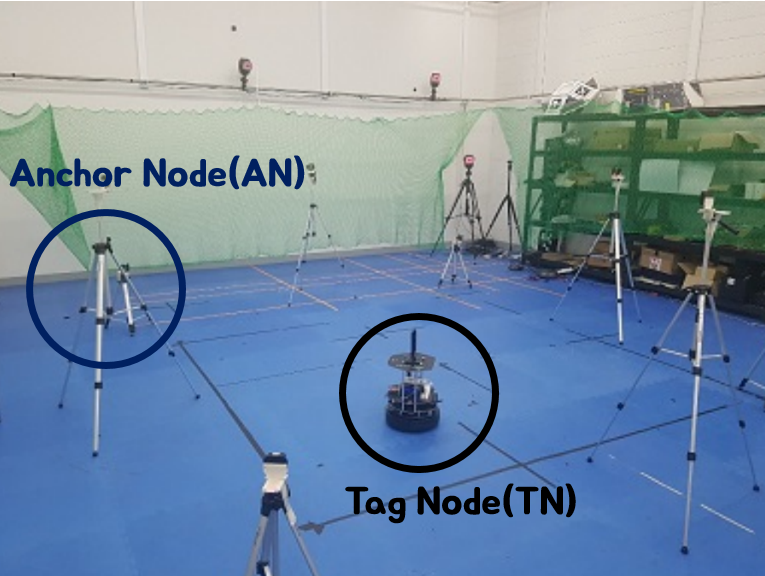
\includegraphics[width=.9\textwidth]{anchor_tag_nodes}
		\label{fig:dataset} 	
		\caption{}
	\end{subfigure}%
	\begin{subfigure}[b]{.25\textwidth}
		\centering
		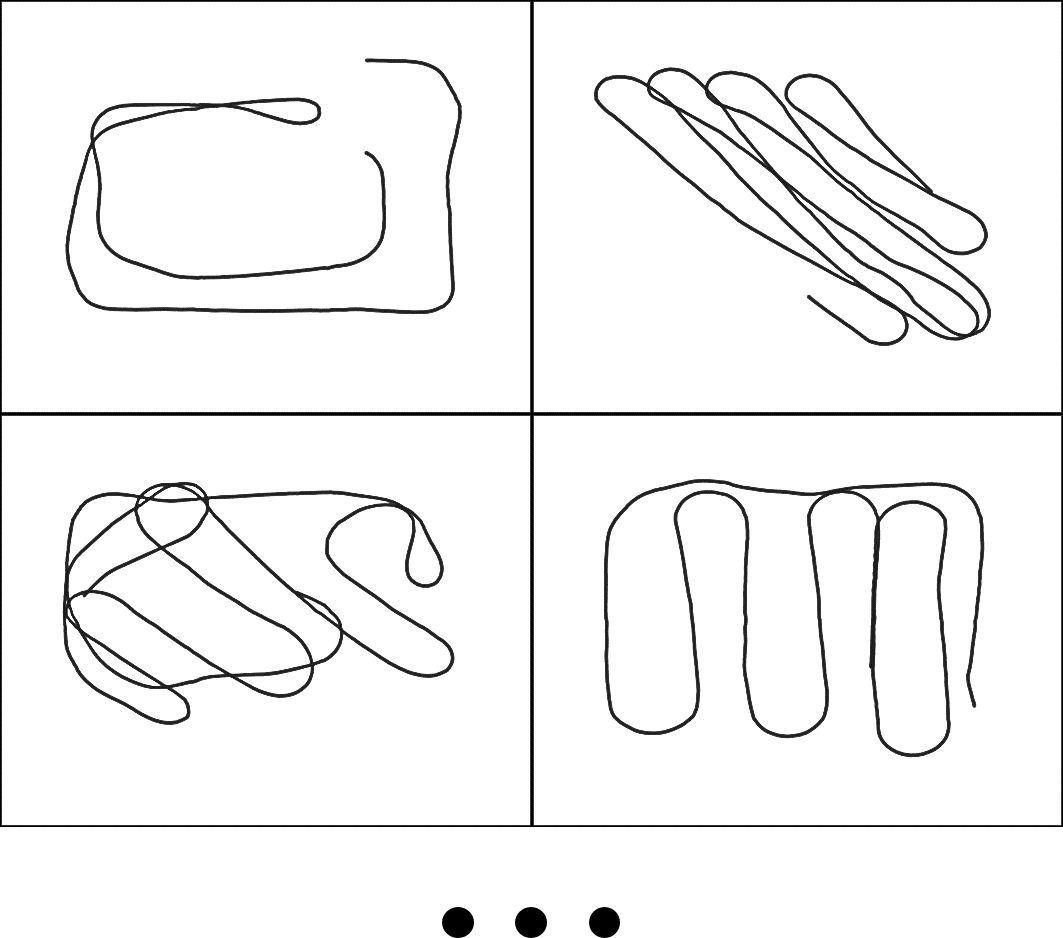
\includegraphics[width=0.9\textwidth]{paths}
		\label{fig:nodes} 	
		\caption{}
	\end{subfigure}%
	\begin{subfigure}[b]{.5\textwidth}
		\centering
		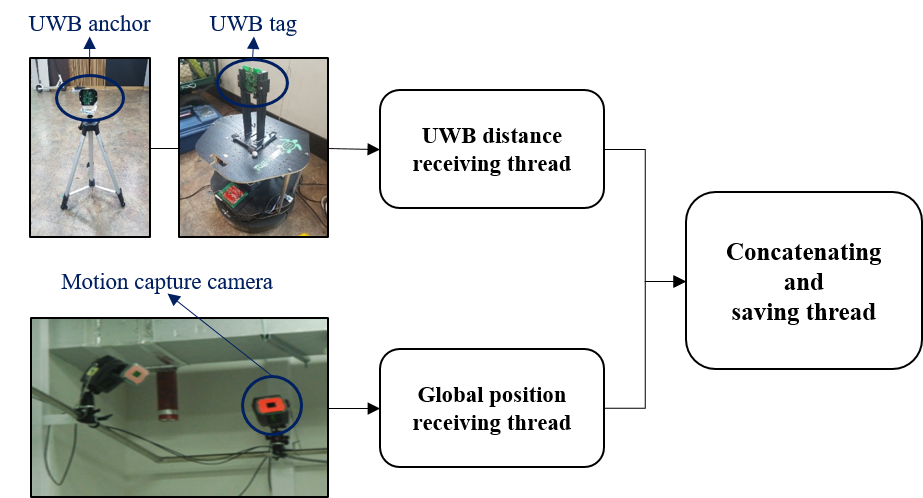
\includegraphics[width=0.9\textwidth]{dataset_process}
		\label{fig:trajectories} 	
		\caption{}
	\end{subfigure}
	\caption{Figures from experiment (a)The anchor and tag nodes (b)Four examples of the trajectory (c) the process that makes dataset}
	\label{fig:experiment}
\end{figure*}
Our experimental system consists of a UWB(ultra wideband) sensor tag and eight anchors that have a UWB transceiver, the motion capture system with 12 cameras, a mobile robot and a small form-factor computer.

UWB sensor anchors are attached to landmarks. These become the end points of the range measurements. The anchor nodes transmit the UWB signal. A UWB sensor tag is attached to a robot. It becomes the opposite side end point of the measurements. The tag node receives the signal and measures the range between two devices. Each UWB transceiver, DW1000 UWB-chip made by Decawave, supports 6 RF bands from 3.5 GHz to 6.5 GHz. It measures in centimeter-level accuracy. Fig. \ref{fig:experiment}(a) shows anchor and tag nodes.

We inference the position of a robot with our network. To train the network and test the results, the ground truths are needed. We get the ground truth by using the motion capture system. The system is Eagle Digital Realtime system of motion analysis corporation that operates with the principle of stereo pattern recognition that is a kind of photogrammetry based on the epipolar geometry and the triangulation methodology. We attach four markers to a robot. The system gives us the location of these markers and has < 1mm accuracy.

A mobile robot used in experiment is iClebo Kobuki from Yujinrobot that has 70 cm/s maximum velocity.The small form-factor computer is a gigabyte Ultra compact PC. Deep learning framework used for our network is pytorch 0.4.0 on python 3.6. The network inferences on the same setting.

The UWB tag is attached to mobile robot that has a small compact computer. The UWB anchors are attached to stands that have two different heights. The anchors are positioned randomly in the square space. As you can see in Fig. \ref{fig:experiment}(b), a mobile robot manually goes on various random trajectories by experimenters.

During the robot is going on, the data is saved in the computer. The distance data used for input data is measured by the UWB sensors. The global position data used for ground truth is measured by the motion capture system. These two kinds of data are paired in a dataset. The computer receives these two kinds of data respectively and syncronizes these by time. To synchronize, we make an independent thread that concatenates and saves these data at the same time. The data is saved at 20Hz frequency. Each trajectory becomes one dataset. All the trajectories are different. Fig. \ref{fig:experiment}(c) shows this process. After collecting whole datasets, we separate the entire dataset to two types, some are the training datasets and others are test datasets.

\subsubsection{Figure Axis labels }
Figure axis labels are often a source of confusion. Use words rather than 
symbols. As an example, write the quantity ``Magnetization,'' or 
``Magnetization M,'' not just ``M.'' Put units in parentheses. Do not label 
axes only with units. As in Fig. 1, for example, write ``Magnetization 
(A/m)'' or ``Magnetization (A$\cdot$m$^{-1}$),'' not just ``A/m.'' Do not label axes with a ratio of quantities and 
units. For example, write ``Temperature (K),'' not ``Temperature/K.'' 

Multipliers can be especially confusing. Write ``Magnetization (kA/m)'' or 
``Magnetization (10$^{3}$ A/m).'' Do not write ``Magnetization 
(A/m)$\,\times\,$1000'' because the reader would not know whether the top 
axis label in Fig. 1 meant 16000 A/m or 0.016 A/m. Figure labels should be 
legible, approximately 8 to 10 point type.

\subsubsection{Subfigure Labels in Multipart Figures and Tables}
Multipart figures should be combined and labeled before final submission. 
Labels should appear centered below each subfigure in 8 point Times New 
Roman font in the format of (a) (b) (c). 

\subsection{File Naming}
Figures (line artwork or photographs) should be named starting with the 
first 5 letters of the author's last name. The next characters in the 
filename should be the number that represents the sequential 
location of this image in your article. For example, in author 
``Anderson's'' paper, the first three figures would be named ander1.tif, 
ander2.tif, and ander3.ps.

Tables should contain only the body of the table (not the caption) and 
should be named similarly to figures, except that `.t' is inserted 
in-between the author's name and the table number. For example, author 
Anderson's first three tables would be named ander.t1.tif, ander.t2.ps, 
ander.t3.eps.

Author photographs should be named using the first five characters of the 
pictured author's last name. For example, four author photographs for a 
paper may be named: oppen.ps, moshc.tif, chen.eps, and duran.pdf.

If two authors or more have the same last name, their first initial(s) can 
be substituted for the fifth, fourth, third$\ldots$ letters of their surname 
until the degree where there is differentiation. For example, two authors 
Michael and Monica Oppenheimer's photos would be named oppmi.tif, and 
oppmo.eps.

\subsection{Referencing a Figure or Table Within Your Paper}
When referencing your figures and tables within your paper, use the 
abbreviation ``Fig.'' even at the beginning of a sentence. Do not abbreviate 
``Table.'' Tables should be numbered with Roman Numerals.

\subsection{Checking Your Figures: The IEEE Graphics Analyzer}
The IEEE Graphics Analyzer enables authors to pre-screen their graphics for 
compliance with IEEE Access standards before submission. 
The online tool, located at
\underline{http://graphicsqc.ieee.org/}, allows authors to 
upload their graphics in order to check that each file is the correct file 
format, resolution, size and colorspace; that no fonts are missing or 
corrupt; that figures are not compiled in layers or have transparency, and 
that they are named according to the IEEE Access naming 
convention. At the end of this automated process, authors are provided with 
a detailed report on each graphic within the web applet, as well as by 
email.

For more information on using the Graphics Analyzer or any other graphics 
related topic, contact the IEEE Graphics Help Desk by e-mail at 
graphics@ieee.org.

\subsection{Submitting Your Graphics}
Because IEEE will do the final formatting of your paper,
you do not need to position figures and tables at the top and bottom of each 
column. In fact, all figures, figure captions, and tables can be placed at 
the end of your paper. In addition to, or even in lieu of submitting figures 
within your final manuscript, figures should be submitted individually, 
separate from the manuscript in one of the file formats listed above in 
Section \ref{formats}. Place figure captions below the figures; place table titles 
above the tables. Please do not include captions as part of the figures, or 
put them in ``text boxes'' linked to the figures. Also, do not place borders 
around the outside of your figures.

\subsection{Color Processing/Printing in IEEE Journals}
All IEEE Transactions, Journals, and Letters allow an author to publish 
color figures on IEEE Xplore\textregistered\ at no charge, and automatically 
convert them to grayscale for print versions. In most journals, figures and 
tables may alternatively be printed in color if an author chooses to do so. 
Please note that this service comes at an extra expense to the author. If 
you intend to have print color graphics, include a note with your final 
paper indicating which figures or tables you would like to be handled that 
way, and stating that you are willing to pay the additional fee.

\section{Conclusion}
A conclusion section is not required. Although a conclusion may review the 
main points of the paper, do not replicate the abstract as the conclusion. A 
conclusion might elaborate on the importance of the work or suggest 
applications and extensions. 

\appendices

Appendixes, if needed, appear before the acknowledgment.

\section*{Acknowledgment}

The preferred spelling of the word ``acknowledgment'' in American English is 
without an ``e'' after the ``g.'' Use the singular heading even if you have 
many acknowledgments. Avoid expressions such as ``One of us (S.B.A.) would 
like to thank $\ldots$ .'' Instead, write ``F. A. Author thanks $\ldots$ .'' In most 
cases, sponsor and financial support acknowledgments are placed in the 
unnumbered footnote on the first page, not here.

\section*{References and Footnotes}

\subsection{References}
References need not be cited in text. When they are, they appear on the 
line, in square brackets, inside the punctuation. Multiple references are 
each numbered with separate brackets. When citing a section in a book, 
please give the relevant page numbers. In text, refer simply to the 
reference number. Do not use ``Ref.'' or ``reference'' except at the 
beginning of a sentence: ``Reference \cite{b3} shows $\ldots$ .'' Please do not use 
automatic endnotes in \emph{Word}, rather, type the reference list at the end of the 
paper using the ``References'' style.

Reference numbers are set flush left and form a column of their own, hanging 
out beyond the body of the reference. The reference numbers are on the line, 
enclosed in square brackets. In all references, the given name of the author 
or editor is abbreviated to the initial only and precedes the last name. Use 
them all; use \emph{et al.} only if names are not given. Use commas around Jr., 
Sr., and III in names. Abbreviate conference titles. When citing IEEE 
transactions, provide the issue number, page range, volume number, year, 
and/or month if available. When referencing a patent, provide the day and 
the month of issue, or application. References may not include all 
information; please obtain and include relevant information. Do not combine 
references. There must be only one reference with each number. If there is a 
URL included with the print reference, it can be included at the end of the 
reference. 

Other than books, capitalize only the first word in a paper title, except 
for proper nouns and element symbols. For papers published in translation 
journals, please give the English citation first, followed by the original 
foreign-language citation See the end of this document for formats and 
examples of common references. For a complete discussion of references and 
their formats, see the IEEE style manual at
\underline{http://www.ieee.org/authortools}.

\subsection{Footnotes}
Number footnotes separately in superscript numbers.\footnote{It is recommended that footnotes be avoided (except for 
the unnumbered footnote with the receipt date on the first page). Instead, 
try to integrate the footnote information into the text.} Place the actual 
footnote at the bottom of the column in which it is cited; do not put 
footnotes in the reference list (endnotes). Use letters for table footnotes 
(see Table \ref{table}).

\section{Submitting Your Paper for Review}

\subsection{Final Stage}
When you submit your final version (after your paper has been accepted), 
print it in two-column format, including figures and tables. You must also 
send your final manuscript on a disk, via e-mail, or through a Web 
manuscript submission system as directed by the society contact. You may use 
\emph{Zip} for large files, or compress files using \emph{Compress, Pkzip, Stuffit,} or \emph{Gzip.} 

Also, send a sheet of paper or PDF with complete contact information for all 
authors. Include full mailing addresses, telephone numbers, fax numbers, and 
e-mail addresses. This information will be used to send each author a 
complimentary copy of the journal in which the paper appears. In addition, 
designate one author as the ``corresponding author.'' This is the author to 
whom proofs of the paper will be sent. Proofs are sent to the corresponding 
author only.

\subsection{Review Stage Using ScholarOne\textregistered\ Manuscripts}
Contributions to the Transactions, Journals, and Letters may be submitted 
electronically on IEEE's on-line manuscript submission and peer-review 
system, ScholarOne\textregistered\ Manuscripts. You can get a listing of the 
publications that participate in ScholarOne at 
\underline{http://www.ieee.org/publications\_standards/publications/}\break\underline{authors/authors\_submission.html}.
First check if you have an existing account. If there is none, please create 
a new account. After logging in, go to your Author Center and click ``Submit 
First Draft of a New Manuscript.'' 

Along with other information, you will be asked to select the subject from a 
pull-down list. Depending on the journal, there are various steps to the 
submission process; you must complete all steps for a complete submission. 
At the end of each step you must click ``Save and Continue''; just uploading 
the paper is not sufficient. After the last step, you should see a 
confirmation that the submission is complete. You should also receive an 
e-mail confirmation. For inquiries regarding the submission of your paper on 
ScholarOne Manuscripts, please contact oprs-support@ieee.org or call +1 732 
465 5861.

ScholarOne Manuscripts will accept files for review in various formats. 
Please check the guidelines of the specific journal for which you plan to 
submit.

You will be asked to file an electronic copyright form immediately upon 
completing the submission process (authors are responsible for obtaining any 
security clearances). Failure to submit the electronic copyright could 
result in publishing delays later. You will also have the opportunity to 
designate your article as ``open access'' if you agree to pay the IEEE open 
access fee. 

\subsection{Final Stage Using ScholarOne Manuscripts}
Upon acceptance, you will receive an email with specific instructions 
regarding the submission of your final files. To avoid any delays in 
publication, please be sure to follow these instructions. Most journals 
require that final submissions be uploaded through ScholarOne Manuscripts, 
although some may still accept final submissions via email. Final 
submissions should include source files of your accepted manuscript, high 
quality graphic files, and a formatted pdf file. If you have any questions 
regarding the final submission process, please contact the administrative 
contact for the journal. 

In addition to this, upload a file with complete contact information for all 
authors. Include full mailing addresses, telephone numbers, fax numbers, and 
e-mail addresses. Designate the author who submitted the manuscript on 
ScholarOne Manuscripts as the ``corresponding author.'' This is the only 
author to whom proofs of the paper will be sent. 

\subsection{Copyright Form}
Authors must submit an electronic IEEE Copyright Form (eCF) upon submitting 
their final manuscript files. You can access the eCF system through your 
manuscript submission system or through the Author Gateway. You are 
responsible for obtaining any necessary approvals and/or security 
clearances. For additional information on intellectual property rights, 
visit the IEEE Intellectual Property Rights department web page at 
\underline{http://www.ieee.org/publications\_standards/publications/}\break\underline{rights/index.html}. 

\section{IEEE Publishing Policy}
The general IEEE policy requires that authors should only submit original 
work that has neither appeared elsewhere for publication, nor is under 
review for another refereed publication. The submitting author must disclose 
all prior publication(s) and current submissions when submitting a 
manuscript. Do not publish ``preliminary'' data or results. The submitting 
author is responsible for obtaining agreement of all coauthors and any 
consent required from employers or sponsors before submitting an article. 
The IEEE Access Department strongly discourages courtesy 
authorship; it is the obligation of the authors to cite only relevant prior 
work.

The IEEE Access Department does not publish conference 
records or proceedings, but can publish articles related to conferences that 
have undergone rigorous peer review. Minimally, two reviews are required for 
every article submitted for peer review.

\section{Publication Principles}
The two types of contents of that are published are; 1) peer-reviewed and 2) 
archival. The Access Department publishes scholarly 
articles of archival value as well as tutorial expositions and critical 
reviews of classical subjects and topics of current interest. 

Authors should consider the following points:

\begin{enumerate}
\item Technical papers submitted for publication must advance the state of knowledge and must cite relevant prior work. 
\item The length of a submitted paper should be commensurate with the importance, or appropriate to the complexity, of the work. For example, an obvious extension of previously published work might not be appropriate for publication or might be adequately treated in just a few pages.
\item Authors must convince both peer reviewers and the editors of the scientific and technical merit of a paper; the standards of proof are higher when extraordinary or unexpected results are reported. 
\item Because replication is required for scientific progress, papers submitted for publication must provide sufficient information to allow readers to perform similar experiments or calculations and 
use the reported results. Although not everything need be disclosed, a paper 
must contain new, useable, and fully described information. For example, a 
specimen's chemical composition need not be reported if the main purpose of 
a paper is to introduce a new measurement technique. Authors should expect 
to be challenged by reviewers if the results are not supported by adequate 
data and critical details.
\item Papers that describe ongoing work or announce the latest technical achievement, which are suitable for presentation at a professional conference, may not be appropriate for publication.
\end{enumerate}

\bibliographystyle{IEEEtran}
% argument is your BibTeX string definitions and bibliography database(s)
\bibliography{./Access_RObib}


\begin{IEEEbiography}[{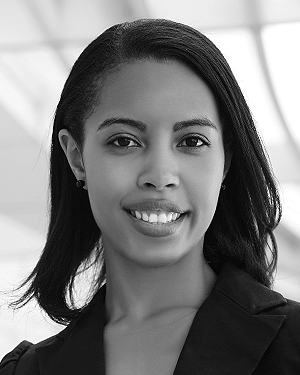
\includegraphics[width=1in,height=1.25in,clip,keepaspectratio]{a1.png}}]{First A. Author} (M'76--SM'81--F'87) and all authors may include 
biographies. Biographies are often not included in conference-related
papers. This author became a Member (M) of IEEE in 1976, a Senior
Member (SM) in 1981, and a Fellow (F) in 1987. The first paragraph may
contain a place and/or date of birth (list place, then date). Next,
the author's educational background is listed. The degrees should be
listed with type of degree in what field, which institution, city,
state, and country, and year the degree was earned. The author's major
field of study should be lower-cased. 

The second paragraph uses the pronoun of the person (he or she) and not the 
author's last name. It lists military and work experience, including summer 
and fellowship jobs. Job titles are capitalized. The current job must have a 
location; previous positions may be listed 
without one. Information concerning previous publications may be included. 
Try not to list more than three books or published articles. The format for 
listing publishers of a book within the biography is: title of book 
(publisher name, year) similar to a reference. Current and previous research 
interests end the paragraph. The third paragraph begins with the author's 
title and last name (e.g., Dr.\ Smith, Prof.\ Jones, Mr.\ Kajor, Ms.\ Hunter). 
List any memberships in professional societies other than the IEEE. Finally, 
list any awards and work for IEEE committees and publications. If a 
photograph is provided, it should be of good quality, and 
professional-looking. Following are two examples of an author's biography.
\end{IEEEbiography}

\begin{IEEEbiography}[{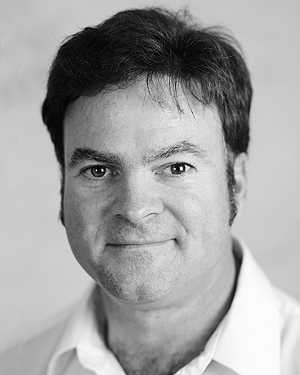
\includegraphics[width=1in,height=1.25in,clip,keepaspectratio]{a2.png}}]{Second B. Author} was born in Greenwich Village, New York, NY, USA in 
1977. He received the B.S. and M.S. degrees in aerospace engineering from 
the University of Virginia, Charlottesville, in 2001 and the Ph.D. degree in 
mechanical engineering from Drexel University, Philadelphia, PA, in 2008.

From 2001 to 2004, he was a Research Assistant with the Princeton Plasma 
Physics Laboratory. Since 2009, he has been an Assistant Professor with the 
Mechanical Engineering Department, Texas A{\&}M University, College Station. 
He is the author of three books, more than 150 articles, and more than 70 
inventions. His research interests include high-pressure and high-density 
nonthermal plasma discharge processes and applications, microscale plasma 
discharges, discharges in liquids, spectroscopic diagnostics, plasma 
propulsion, and innovation plasma applications. He is an Associate Editor of 
the journal \emph{Earth, Moon, Planets}, and holds two patents. 

Dr. Author was a recipient of the International Association of Geomagnetism 
and Aeronomy Young Scientist Award for Excellence in 2008, and the IEEE 
Electromagnetic Compatibility Society Best Symposium Paper Award in 2011. 
\end{IEEEbiography}

\begin{IEEEbiography}[{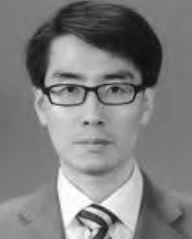
\includegraphics[width=1in,height=1.25in,clip,keepaspectratio]{a3.png}}]{Third C. Author, Jr.} (M'87) received the B.S. degree in mechanical 
engineering from National Chung Cheng University, Chiayi, Taiwan, in 2004 
and the M.S. degree in mechanical engineering from National Tsing Hua 
University, Hsinchu, Taiwan, in 2006. He is currently pursuing the Ph.D. 
degree in mechanical engineering at Texas A{\&}M University, College 
Station, TX, USA.

From 2008 to 2009, he was a Research Assistant with the Institute of 
Physics, Academia Sinica, Tapei, Taiwan. His research interest includes the 
development of surface processing and biological/medical treatment 
techniques using nonthermal atmospheric pressure plasmas, fundamental study 
of plasma sources, and fabrication of micro- or nanostructured surfaces. 

Mr. Author's awards and honors include the Frew Fellowship (Australian 
Academy of Science), the I. I. Rabi Prize (APS), the European Frequency and 
Time Forum Award, the Carl Zeiss Research Award, the William F. Meggers 
Award and the Adolph Lomb Medal (OSA).
\end{IEEEbiography}

\EOD

\end{document}
